\documentclass{article}
\usepackage{hyperref}
\usepackage{listings}
\usepackage{color}
\usepackage{xcolor}
\usepackage{geometry}
\usepackage{graphicx}
\usepackage{amsmath}
\usepackage{caption}
\usepackage{subcaption}
\geometry{margin=1in}
\pdfminorversion=6

\newcommand\TODO[1]{\textcolor{red}{TODO: #1}}

\newcommand\header[2]{
    \begin{center}
        {\large
        UCSD CSE 272 Assignment #1: \\
        \vspace{0.3cm}
        \Large
        #2}
    \end{center}
}

\definecolor{dkgreen}{rgb}{0,0.6,0}
\definecolor{gray}{rgb}{0.5,0.5,0.5}
\definecolor{mauve}{rgb}{0.58,0,0.82}
\lstset{frame=tb,
        aboveskip=3mm,
        belowskip=3mm,
        showstringspaces=false,
        columns=flexible,
        basicstyle={\small\ttfamily},
        numbers=none,
        numberstyle=\tiny\color{gray},
        keywordstyle=\color{blue},
        commentstyle=\color{dkgreen},
        stringstyle=\color{mauve},
        breaklines=true,
        breakatwhitespace=true,
        tabsize=2
}

\hypersetup{colorlinks=true}


\begin{document}

\header{1}{Volumetric Path Tracing}

\begin{figure}[h]
    \includegraphics[width=\linewidth]{imgs/colored_smoke.png}
    \caption{A heterogeneous volume with spectrally varying density over space, rendered with multiple-scattering. Smoke data generated using Wenzel Jakob's \href{http://www.mitsuba-renderer.org/misc.html}{fsolver}.}
    \label{fig:gallery}
\end{figure}

In this homework, we will build a volumetric path tracers that can handle scattering and absorption inside participating media inside lajolla. We will split the development into 6 steps and build 6 volumetric path tracers, each has more features than the previous ones.\footnote{This approach is inspired by Steve Marschner's \href{https://www.cs.cornell.edu/courses/cs6630/2015fa/notes/10volpath.pdf}{course note} on volumetric path tracing.} Your $n$-th volumetric path tracer should be able to render all scenes the $(n-1)$-th one can handle. If you want, you can only submit the final volumetric path tracer and let all the rest call the final code. This process is for helping you to slowly and steadily build up your rendering algorithm.

Participating media are volumes with many infinitesimal particles absorbing and scattering lights. Given a ray inside the volume parametrized by distance $\mathbf{p}(t)$, the radiance along the ray is modelled by the \emph{radiative transfer equation}:
\begin{equation}
\frac{\mathrm{d}}{\mathrm{d}t} L(\mathbf{p}(t), \omega) = -(\sigma_a(\mathbf{p}(t)) + \sigma_s(\mathbf{p}(t))) L(\mathbf{p}(t), \omega) + \sigma_a L_e(\mathbf{p}(t), \omega) + \sigma_s(\mathbf{p}(t)) \int_{S^2} \rho(\mathbf{p}(t), \omega, \omega') L(\mathbf{p}(t), \omega') \mathrm{d}\omega',
\label{eq:rte}
\end{equation}
where $L$ is the radiance, $\sigma_a$ is the \emph{absorption coefficient}, $\sigma_s$ is the \emph{scattering coefficient}, $L_e$ is the (volumetric) emission, $\rho$ is the \emph{phase function} that is skin to BSDF in surface rendering, and $S^2$ is the spherical domain.

This looks a bit scary, so let's break it down. From now on we'll drop the arguments for $\sigma_a$ and $\sigma_s$, but in general they can still be spatially varying. The radiative transfer equation is made of four components: \textbf{absorption}, \textbf{emission}, \textbf{in-scattering}, and \textbf{out-scattering}. Absorption and emission handles particles that absorb and emit lights:
\begin{equation}
\frac{\mathrm{d}}{\mathrm{d}t} L_a(\mathbf{p}(t), \omega) = -\sigma_a L_a(\mathbf{p}(t), \omega) + \sigma_a L_e(\mathbf{p}(t), \omega).
\end{equation}
Notice how this is just a simple linear ordinary differential equation $x' = ax + b$, where $\sigma_a$ attenuates lights and $L_e$ is the gain.

The in-scattering accounts for all the lights bounces between the particles along the ray, just like the surface rendering equation:
\begin{equation}
\frac{\mathrm{d}}{\mathrm{d}t} L_{is}(\mathbf{p}(t), \omega) = \sigma_s \int_{S^2} \rho(\mathbf{p}(t), \omega, \omega') L(\mathbf{p}(t), \omega') \mathrm{d}\omega'.
\end{equation}

However, the light does not just bounce \emph{into} the ray, it also bounces \emph{out}. That's what the out-scattering considers:
\begin{equation}
\frac{\mathrm{d}}{\mathrm{d}t} L_{os}(\mathbf{p}(t), \omega) = -\sigma_s L_{os}(\mathbf{p}(t)).
\end{equation}

Combining all these three components, we get the full radiative transfer equation (Equation~\ref{eq:rte}). Notice that the full radiative transfer equation is also like a linear ODE: $-(\sigma_a + \sigma_s) L$ attenuates light, and $L_e$ and the spherical integral are the gain that makes things brighter. For this reason, we often let $\sigma_t = \sigma_a + \sigma_s$ and call it the \emph{extinction coefficient}.

We'll start from a very simplified version of the radiative transfer equation, then slowly handle more complex situations. To make things simpler, we will throughout assume our medium does not emit light itself: it will receive lighting from other surfaces in the scene.

Before that, let's introduce lajolla's data structures for storing the participating media.

\section{Lajolla's participating media data structures and interfaces}
\begin{figure}
    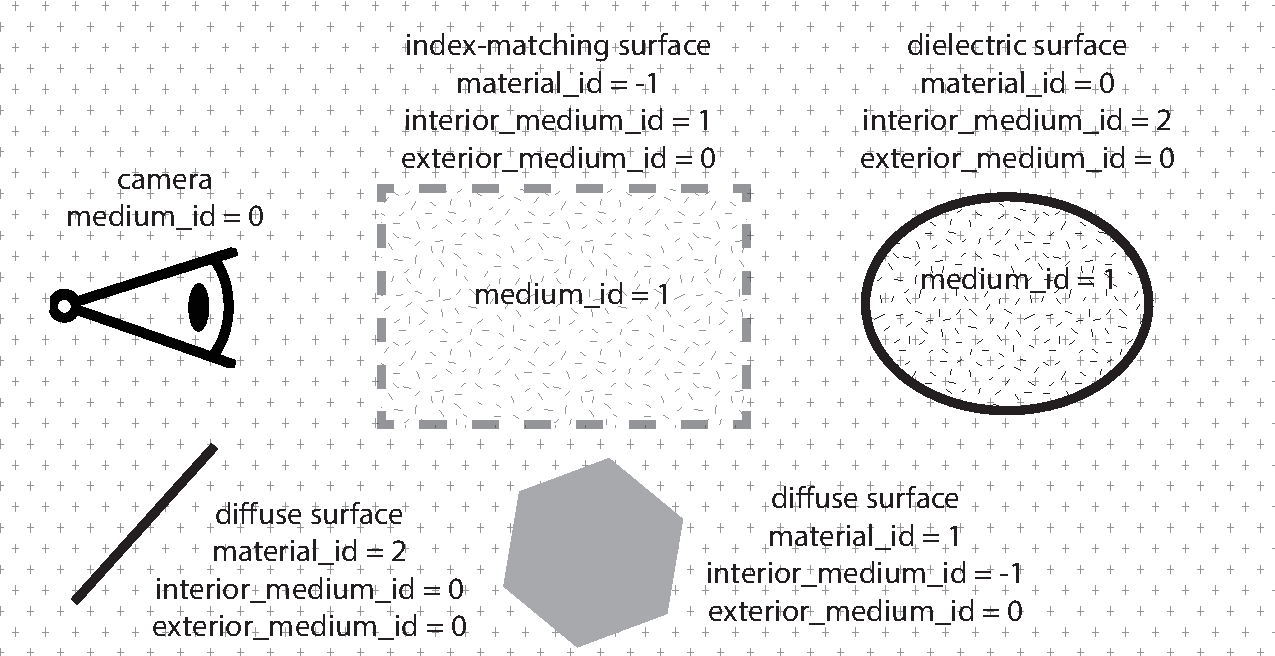
\includegraphics[width=\linewidth]{imgs/media.pdf}
    \caption{Lajolla assumes that media are separated by closed surface boundaries. At the object surface, we store the ID of the interior and exterior media (if either of them is vaccum, set the ID to \lstinline{-1}). The outmost medium is specified at the camera (and can be accessed through \lstinline{camera.medium_id}). A surface can be \emph{index-matching} meaning that light just pass through without changing direction or losing energy. In this case, the \lstinline{material_id} of the surface is set to \lstinline{-1}. A surface can also be transmissive. In this case, it is assigned a transmissive material like \lstinline{roughdielectric}.}
    \label{fig:data_structure}
\end{figure}

\paragraph{The Medium struct in lajolla.} Lajolla's medium interface is for querying the media parameters $\sigma_a$, $\sigma_s$, phase function $\rho$, and the \emph{majorant} which is the upper bound of the extinction coefficient $\sigma_t = \sigma_a + \sigma_s$ -- we will need the majorant in our final renderer. 
\begin{lstlisting}[language=c++]
struct MediumBase {
    PhaseFunction phase_function;
};

struct HomogeneousMedium : public MediumBase {
    Spectrum sigma_a, sigma_s;
};

struct HeterogeneousMedium : public MediumBase {
    VolumeSpectrum albedo, density;
};

using Medium = std::variant<HomogeneousMedium, HeterogeneousMedium>;

/// the maximum of sigma_t = sigma_s + sigma_a over the whole space
Spectrum get_majorant(const Medium &medium, const Ray &ray);
Spectrum get_sigma_s(const Medium &medium, const Vector3 &p);
Spectrum get_sigma_a(const Medium &medium, const Vector3 &p);

inline PhaseFunction get_phase_function(const Medium &medium) {
    return std::visit([&](const auto &m) { return m.phase_function; }, medium);
}
\end{lstlisting}
You will need these functions to obtain the necessary quantities in the homeworks.

A \lstinline{HomogeneousMedium} should be straightforward: it contains constant $\sigma_a$ and $\sigma_s$.
We will talk more about \lstinline{HeterogeneousMedium} and \lstinline{PhaseFunction} later.

Lajolla assumes that the media are separated by surface boundaries (Figure~\ref{fig:data_structure}). It's up to the upstream user to make sure they are consistent to each other and the surfaces are closed (if they are not, the results are undefined).\footnote{Modern production volume renderers have paid special attention to make sure the renderers can handle all sorts of inputs, including nested volumes. See \href{here}{https://graphics.pixar.com/library/ProductionVolumeRendering/index.html} for more information.} 

In the scene file, each objects are marked with corresponding exterior and interior media:
\begin{lstlisting}[language=xml]
    <medium type="homogeneous" id="medium">
        <rgb name="sigmaA" value="0.5 0.5 0.5"/>
        <rgb name="sigmaS" value="0.0 0.0 0.0"/>
        <float name="scale" value="3"/>
    </medium>

    <shape type="sphere">
        <!-- ...  -->
        <ref name="exterior" id="medium"/>
    </shape>

    <sensor type="perspective">
        <!-- ... -->

        <ref id="medium"/>
    </sensor>
\end{lstlisting}

The \lstinline{Medium}s are stored in \lstinline{scene.media} which you can access through \lstinline{scene.media[medium_id]}. The \lstinline{intersection} routine in lajolla returns a \lstinline{PathVertex} object which contains relevant information of the intersection:
\begin{lstlisting}[language=c++]
struct PathVertex {
    Vector3 position;
    Vector3 geometry_normal;
    // ...
    int shape_id = -1;
    int primitive_id = -1; // For triangle meshes. This indicates which triangle it hits.
    int material_id = -1;

    // If the path vertex is inside a medium, these two IDs
    // are the same.
    int interior_medium_id = -1;
    int exterior_medium_id = -1;
};
\end{lstlisting}

\section{Single absorption-only homogeneous volume}
\begin{figure}
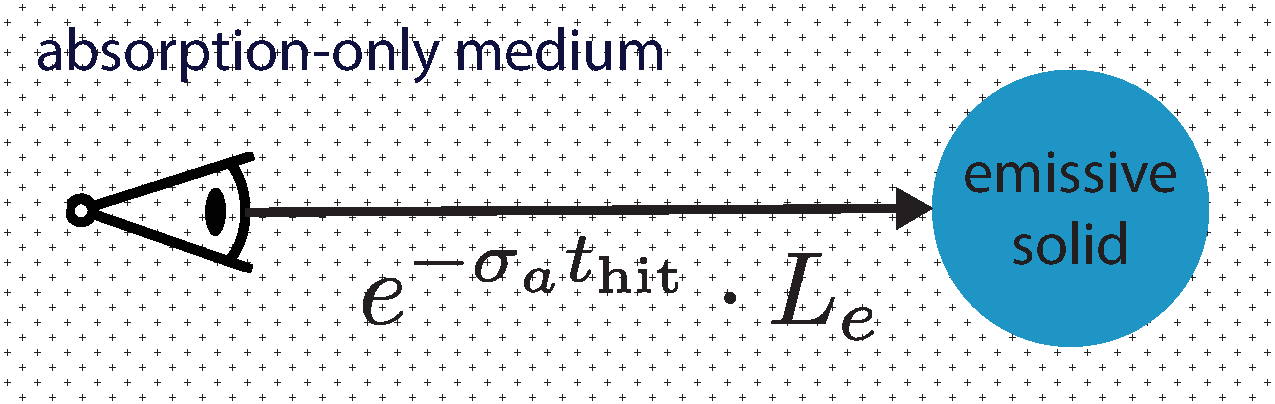
\includegraphics[width=\linewidth]{imgs/absorption_medium.pdf}
\caption{The setup of our first volumetric renderer.}
\label{fig:volpath1_illustration}
\end{figure}
\begin{figure}
\caption{Our first volume rendering.}
\label{fig:volpath1}
\end{figure}

Our first volume renderer will make four assumptions:
\begin{itemize}
    \item There is only a single, homogeneous ($\sigma_a$ and $\sigma_s$ are constants over space) volume.
    \item The volume does not scatter light: $\sigma_s = 0$.
    \item The surfaces in the scene only emit lights (with intensity $L_e$) and do not reflect/transmit lights.
\end{itemize}

Under these assumptions, the radiative transfer equation becomes
\begin{equation}
\frac{\mathrm{d}}{\mathrm{d}t} L_a(\mathbf{p}(t), \omega) = -\sigma_a L_a(\mathbf{p}(t), \omega),
\end{equation}
and we know $L_a(\mathbf{p}(t_{\text{hit}}), \omega) = L_e$ where $t_{\text{hit}}$ is the distance between the origin of the ray and the emissive surface. 

This ordinary differential equation has a simple closed form:
\begin{equation}
L_a(\mathbf{p}(0), \omega) = \exp\left(-\sigma_a t_{\text{hit}} \right) L_e.
\end{equation}
Figure~\ref{fig:volpath1_illustration} illustrates the setup. In volume rendering the exponential term
$\exp\left(-\sigma_a t_{\text{hit}} \right)$ is often called the ``transmittance''.

Our rendering algorithm is as follows (in Python-style pseudo code).
\begin{lstlisting}[language=python]
def L(screen_pos):
  camera_ray = sample_primary(camera, screen_pos)
  isect = intersect(scene, camera_ray)
  if isect:
    transmittance = exp(-sigma_a * t)
    Le = 0
    if is_light(isect):
      Le = isect.Le
    return transmittance * Le
  return 0
\end{lstlisting}

\paragraph{Task (15\%).} You will implement the algorithm above in the \lstinline{vol_path_tracing_1} function in \lstinline{vol_path_tracing.h}. You might want to first look at the surface path tracing code in \lstinline{path_tracing.h} to understand lajolla's API better. 

\end{document}